%!TeX root = ../index.tex

\section{Schema Management}\label{sec:schema-management}

This section examines the problem domain of schema management by analyzing an example use case and parallel use cases from academic literature.
Before though, it provides essential information regarding the two prominent technologies of these use cases: Apache Kafka and Apache Avro.
Building on the analysis, the subsequent text deduces a definition of schema management and the characteristics of a schema management solution.

\subsection{Messaging Technologies}

\subsubsection{Apache Kafka}

The LinkedIn employees \citeauthor{kreps_kafka_2011} introduced their new \enquote{Event Streaming Platform} \emph{Kafka} in \citeyear{kreps_kafka_2011} \parencite{kreps_kafka_2011}.
Over a decade later, the project has since joined the Apache foundation and \enquote{[m]ore than 80\% of all Fortune 100 companies trust, and use [it]} \parencite{apache_software_foundation_apache_nodate}.

\citeauthor{kreps_kafka_2011} describe Kafka as \enquote{[\ldots] a novel messaging system for log processing [\ldots] that combines the benefits of traditional log aggregators and messaging systems.} \parencite{kreps_kafka_2011}.
The solution has an \gls{api} that is similar to traditional \gls{mom}, yet it persists messages in an append-only log structure on the hard drive.
This detail allows Kafka to not only stream data in near real-time but persist large amounts of it for online analytical processing.
In addition to that, Kafka features partitioning and replication mechanisms which make it highly available and scalable. \parencite{kreps_kafka_2011}

Kafka is not only useful for processing the kinds of log data that are proposed by \citeauthor{kreps_kafka_2011}: activity (e.~g. user logins, clicks, \enquote{likes}, \ldots) and operational data (e.~g. \gls{cpu} or disk utilization, \gls{http} requests, \ldots) \parencite{kreps_kafka_2011}.
\citeauthor{stopford_designing_2018}, for example, outlines how the entire state management and internal communication of a business application can be based on Apache Kafka.
His design implements concepts from the \gls{ddd} community like Event Sourcing \parencite{fowler_event_sourcing_2005} and \gls{cqrs} \parencite{fowler_cqrs_2011} with Apache Kafka's log-based messaging at the center \parencite{stopford_designing_2018}.
The potential use cases of Apache Kafka are therefore plentiful.

\subsubsection{Apache Avro}

Apache Avro provides the ability to define rich data structures and interfaces for \glspl{rpc} as schema documents.
On top of that, it offers an efficient binary data format for serialization.
Listing \ref{lst:avro-schema-person} shows an example for an Avro schema describing a person entity.
\parencite{apache_software_foundation_apache_2021}

\begin{listing}[H]
  \inputminted{json}{assets/src/Person.avsc}
  \caption{Avro Schema of a Person Entity}\label{lst:avro-schema-person}
\end{listing}

Avro's design assumes that applications that (de)-serialize data have access to the data's schema.
That is one of the reasons why the format is so efficient.
It does not need to include type information in the serialized data.
Avro's support for schema evolution builds upon this assumption.
If an application attempts to de-serialize data encoded in Avro binary, it requires both the schema with which the data was written and the schema which the application understands.
These schemas are called the \emph{writer} and the \emph{reader} schema respectively.
In the simplest case, these schemas might be equal.
Nevertheless, Avro also supports de-serializing data with a reader schema different from the writer schema.
Although, the de-serialization will only succeed if both schemas are still \emph{compatible}.
\parencite{apache_software_foundation_apache_2021}

If, for example, the reader schema had an additional field without a default value.
It would be an incompatible change because Avro would not be able to infer a value for the additional field.
On the other hand, if the field had a default value, the de-serialization would succeed.
\citeauthor{kreps_kafka_2011} chose Apache Avro as the serialization protocol for their message payloads due to its efficiency and schema evolution capabilities \parencite{kreps_kafka_2011}. 

\subsection{The Case for Schema Management}

This section examines the problem domain that schema management addresses.
It does so by analyzing a hypothetical \gls{is} design for a web-shop application.
The analysis serves as a basis for a definition of schema management and the characteristics of schema management solutions.

The design features a set of microservice applications hosted on virtualized infrastructure.
It employs Apache Kafka as a \gls{mom} to facilitate the communication between the microservices.
Cross-functional teams develop and deploy each microservice with a great degree of independence.
The teams use Apache Avro to define schemas for the messages that the microservices send and receive.
They have integrated it into the services to serialize the payload of a message into Avro's binary format before they send it to Kafka.

\begin{figure}[H]
  \centering
  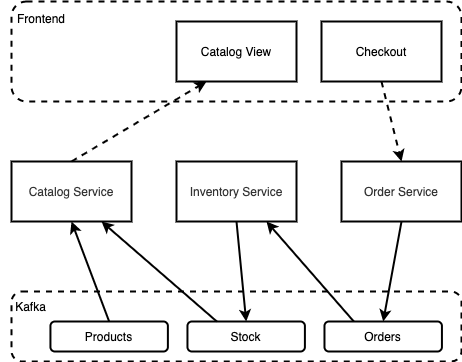
\includegraphics[width=0.8\linewidth]{webshop.drawio.png}
  \caption{Simplified Webshop Design Using Apache Kafka}\label{fig:webshop}
\end{figure}


\subsection{Definition of Schema Management}

\subsection{Characteristics of Schema Management Solutions}
